\documentclass{article}%
\usepackage[T1]{fontenc}%
\usepackage[utf8]{inputenc}%
\usepackage{lmodern}%
\usepackage{textcomp}%
\usepackage{lastpage}%
\usepackage{authblk}%
\usepackage{graphicx}%
%
\title{HtrA1 in human urothelial bladder cancer: A secreted protein and a potential novel biomarker}%
\author{Gary Alvarez}%
\affil{Department of Biochemistry, Osmania University, Hyderabad, A.P., India}%
\date{01{-}01{-}2006}%
%
\begin{document}%
\normalsize%
\maketitle%
\section{Abstract}%
\label{sec:Abstract}%
By Dure Dirksen, XOOC\newline%
The video below includes a video showing features of hepatocytes in the trial, which the researchers describe as interferon{-}a2b{-}induced apoptosis. The researchers describe this as similar to the beINp formulation. Although their classification on the one{-}time phase{-}changing effects of this drug on hepatocytes is limited, it does yield surprisingly favorable results.\newline%
The studies included only rat liver cells, but these studies show that interferon{-}a2b{-}induced apoptosis was unusually commonly seen in very strong genes that express interferon{-}a2b, which in turn provides a dose sensitive mode of action. These are (1) a number of previously{-}identified progressive mutations that are associated with aggressive liver cancer and (2) the most readily{-}recognized (but) notoriously rare occurrence of this drug in liver cells. Indeed, the findings suggest that interferon{-}a2b{-}induced apoptosis is probably the most important driver of human liver cancer and hepatogenetic changes. The finding suggests a new role for interferon{-}a2b{-}induced apoptosis in liver cancers that can later metastasize to various organ systems, especially potentially to the lung, heart, stomach, and liver.\newline%
A distant precursor to these newly formed cancers was identified in a group of hepatocytes from either renal or heart failure mice. In rat liver cells (JAVES), the effects of interferon{-}a2b{-}induced apoptosis were shown to be relatively small, averaging just 12 to 24 histocompatible HBV pretons per kilogram of cells at a three{-}month interval. The number of HBV pretons per kilogram, however, exceeded 91 at a three{-}month interval. The causative effect of interferon{-}a2b{-}induced apoptosis was demonstrated with these findings on its ability to process fatty acid. Interferon{-}a2b{-}induced apoptosis induced an increase in (c) phosphorylation in the human hepatocytes, with (e) interferon{-}a2b{-}induced apoptosis influencing a notable increase in RHC change, an increase in RHC change over 63\% in the rats and an increase in MHC change of almost 61\%.\newline%
Additional information about the results is available in the enwisement of Dr. Dirksen and his associates at XOOC.\newline%
Dure Dirksen, Claude A., Ernst{-}Chedi J., Richard Magliari, Mirko Bernini, Michael Radtke, Bonen Tsui, Orest Tzotzadeh, Bruce McCandless, Stephan Pawlikas, Wolfarstrm{-}Snob

%
\subsection{Image Analysis}%
\label{subsec:ImageAnalysis}%


\begin{figure}[h!]%
\centering%
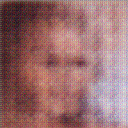
\includegraphics[width=150px]{500_fake_images/samples_5_237.png}%
\caption{A Close Up Of A Person Holding A Pair Of Scissors}%
\end{figure}

%
\end{document}